% -*- program: xelatex -*-

\documentclass{beamer}

\usefonttheme{professionalfonts} % using non standard fonts for beamer
\usepackage{fontspec}
\setmainfont{Arial}
\usefonttheme[onlymath]{serif}
\usepackage{datetime}

\title{\LARGE A beamer presentation\\using HUJI's design language:}
\subtitle{easier than you think} % optional
\newdate{presentationdate}{31}{12}{2017}
\author{Author Name}
\institute{Hogwarts School of Witchcraft and Wizardry} % optional

\usetheme{huji}%
\pgfplotsset{compat=1.16}

\begin{document}
% GreenAndPurple, GreyAndAzure, RedAndLightBlue, GoldAndSilver
\hujicolortheme{GreenAndPurple}

\begin{frame}[noframenumbering]
\titlepage
\end{frame}

\section{section 1}

\begin{frame} 
\frametitle{There Is No Largest Prime Number} 
\framesubtitle{The proof uses \textit{reductio ad absurdum}.} 
\begin{theorem}
There is no largest prime number. \end{theorem} 
\begin{enumerate} 
\item Suppose $p$ were the largest prime number. 
\item Let $q$ be the product of the first $p$ numbers. 
\item Then $q+1$ is not divisible by any of them. 
\item But $q + 1$ is greater than $1$, thus divisible by some prime number not in the first $p$ numbers.
\end{enumerate}
\end{frame}

\begin{frame}{Bullet Points}

\begin{columns}[T]
\begin{column}{0.45\textwidth}
\begin{itemize}
\item hebrew
\item university
\item of
\item jerusalem
\end{itemize}
\end{column}
\begin{column}{0.45\textwidth}
\includegraphics[height=0.6\textheight]{hujilogo.pdf}
\end{column}
\end{columns}

\end{frame}

\section{middle}

\begin{frame}{equations}
\centering
\vspace{-1em}
\[
\cos (2\theta) = \cos^2\! \theta - \sin^2\! \theta
\]

\vspace{1em}
and
\vspace{1em}
\[
A_{m,n} = 
 \begin{pmatrix}
  a_{1,1} & a_{1,2} & \cdots & a_{1,n} \\
  a_{2,1} & a_{2,2} & \cdots & a_{2,n} \\
  \vdots  & \vdots  & \ddots & \vdots  \\
  a_{m,1} & a_{m,2} & \cdots & a_{m,n} 
 \end{pmatrix}
\]
\end{frame}

\begin{frame}{inline math}
Lorem ipsum dolor sit amet, consectetur adipiscing elit $(ax^2+bx+c=0)$.
Ut in nulla cursus, fermentum eros at, pulvinar neque. Nullam nec scelerisque erat.
Quisque vitae dolor ex. 
Sed sit amet venenatis ligula. $(-b\pm\sqrt{b^2-4ac})/2a$
Nam dictum sapien orci, nec laoreet eros finibus quis.
Suspendisse dictum nisl quam. Aenean porta aliquam auctor.
\end{frame}

\section{conclusion}

\begin{frame}{evolve}
Show a sequence of images, all must have the same size:
\begin{center}
\includegraphics<1>[width=0.6\columnwidth]{evolve1}%
\includegraphics<2>[width=0.6\columnwidth]{evolve2}%
\includegraphics<3>[width=0.6\columnwidth]{evolve3}%
\end{center}
\end{frame}

\begin{frame}{tikz+beamer}
\centering
\onslide<1->{
    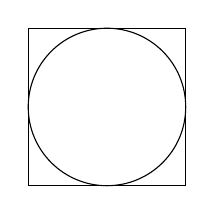
\begin{tikzpicture}
      \draw (0,0) rectangle (2,2);
      \onslide<2->{
          \draw (1,1) circle [radius=1cm];
      }
    \end{tikzpicture}
  }
  \onslide<3->{
    Comment
  }
\end{frame}


\end{document}